\section{Numerical Results}
\label{sec:results}

Our code is written in \texttt{C++} using \texttt{MPI} and \texttt{OpenMP} and is freely available on github (url withheld for review) under an MIT license. 
All experiments were conducted on the RMACC Summit Supercomputer at the University of Colorado, Boulder (via XSEDE). Each node has 24 cores and it uses Intel Xeon E5-2680 with $4.84GB$ of memory per core. All experiments were run in the hybrid \texttt{MPI+OpenMP} mode. 


For these experiments for \mm~ we have multiplied a banded matrix with itself, assuming that the matrix is being multiplied with a separate matrix, so not using any information from the left-hand side matrix for the right-hand side one.

Figure\ref{fig:strong1} is the strong scaling for five banded matrices of the same size ($192k$), but with different bandwidth. The legend shows the density ($\frac{nonzero}{size^2}$) of each matrix. Our solver scales consistently for different density values. There is no data in the plot for the matrix with density $0.02$ on $24$ processors because it was too big to fit in the memory of one node.

\begin{figure}[tbh]
 \centering
 \Description{Description}
 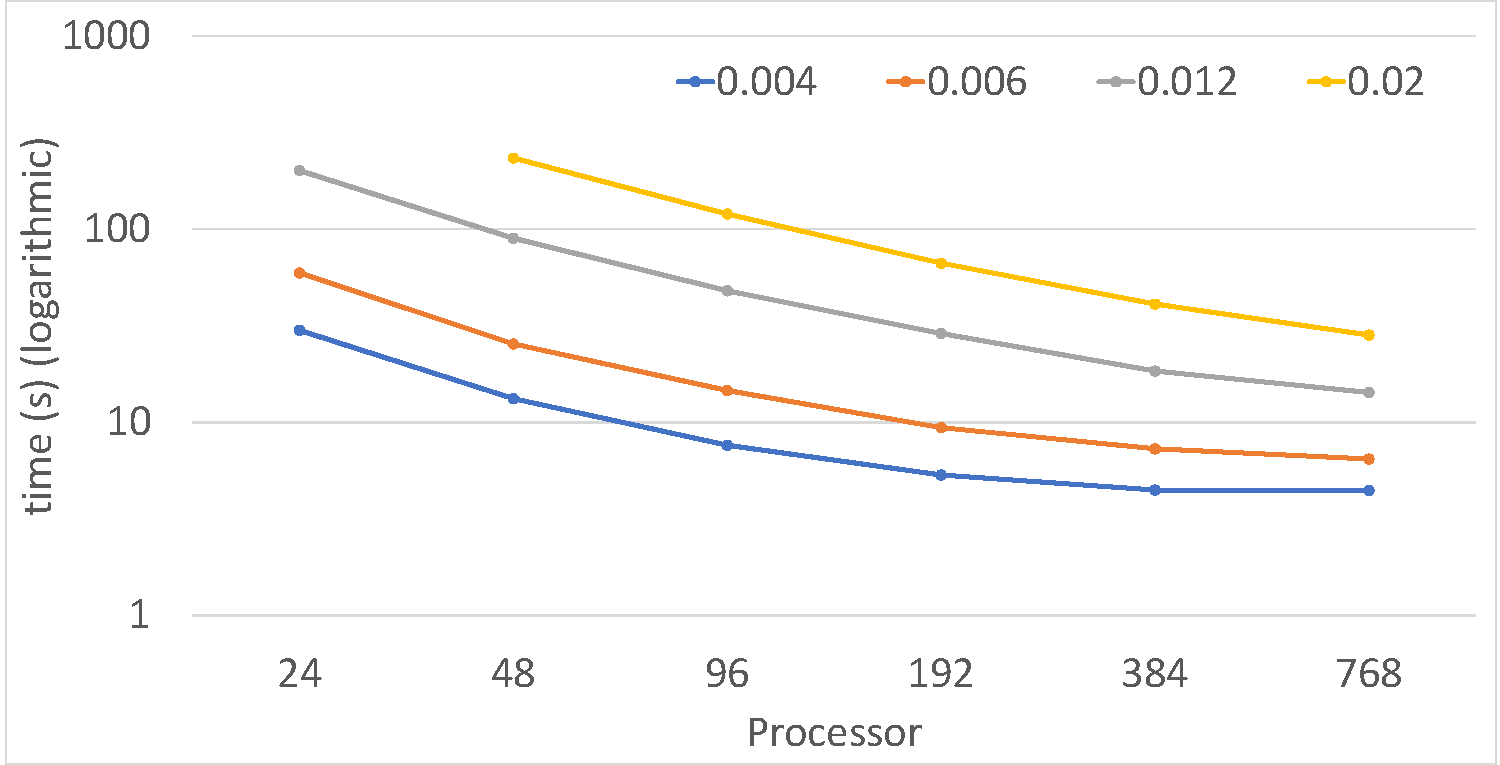
\includegraphics[width=8.5cm,height=4.9cm]{./figures/strong_size.pdf}
 \caption{Strong scaling for five banded matrices of the same size (192k), but with different bandwidth. The legend shows the density ($\frac{nonzero}{size^2}$) of each matrix.}
 \label{fig:strong1}
\end{figure}

Figure\ref{fig:size_vs_nnz} compares the scaling time for when we split the matrices based on matrix size and when we split based on number of nonzeros. The one that uses the matrix size is more scalable, especially for denser matrices.

\begin{figure}[tbh]
 \centering
 \Description{Description}
 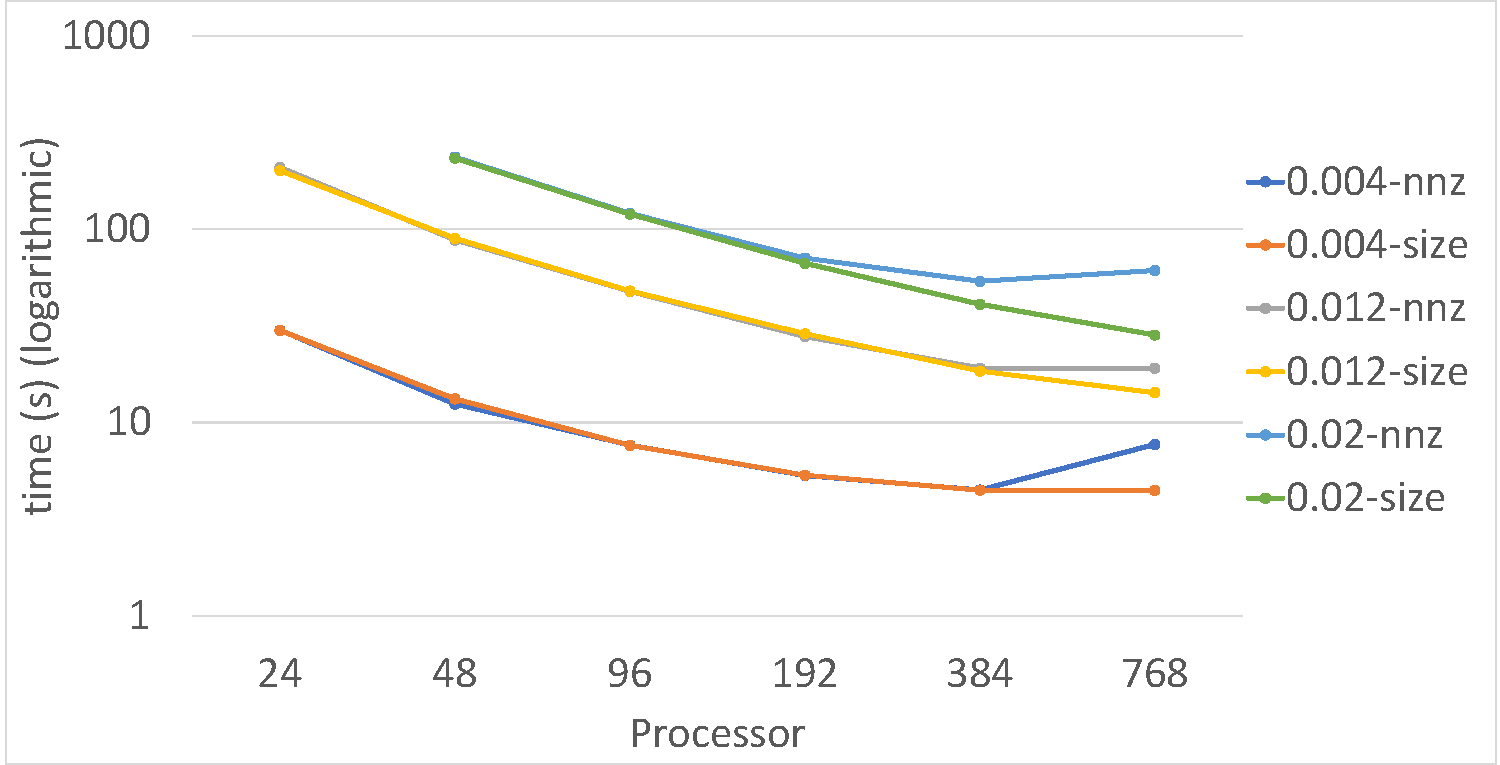
\includegraphics[width=8.5cm,height=4.4cm]{./figures/strong_size_vs_nnz.pdf}
 \caption{Comparison of the the strong scaling when using two different splitting strategies: based on matrix size and based on number of nonzeros. The legend shows the density of each matrix.}
 \label{fig:size_vs_nnz}
\end{figure}

Figure\ref{fig:petsc1} compares the strong scaling between our solver with PETSc. For the matrices with lower density (more sparse) PETSc performs better when using higher number of processes, but for denser matrices our solver is faster. In multigrid hierarchy, the coarse matrices get denser as we go to lower levels, so it becomes expensive to perform \mm~ at those levels and having an efficient matrix-matrix product will improve the setup cost significantly.

\begin{figure}[tbh]
 \centering
 \Description{Description}
 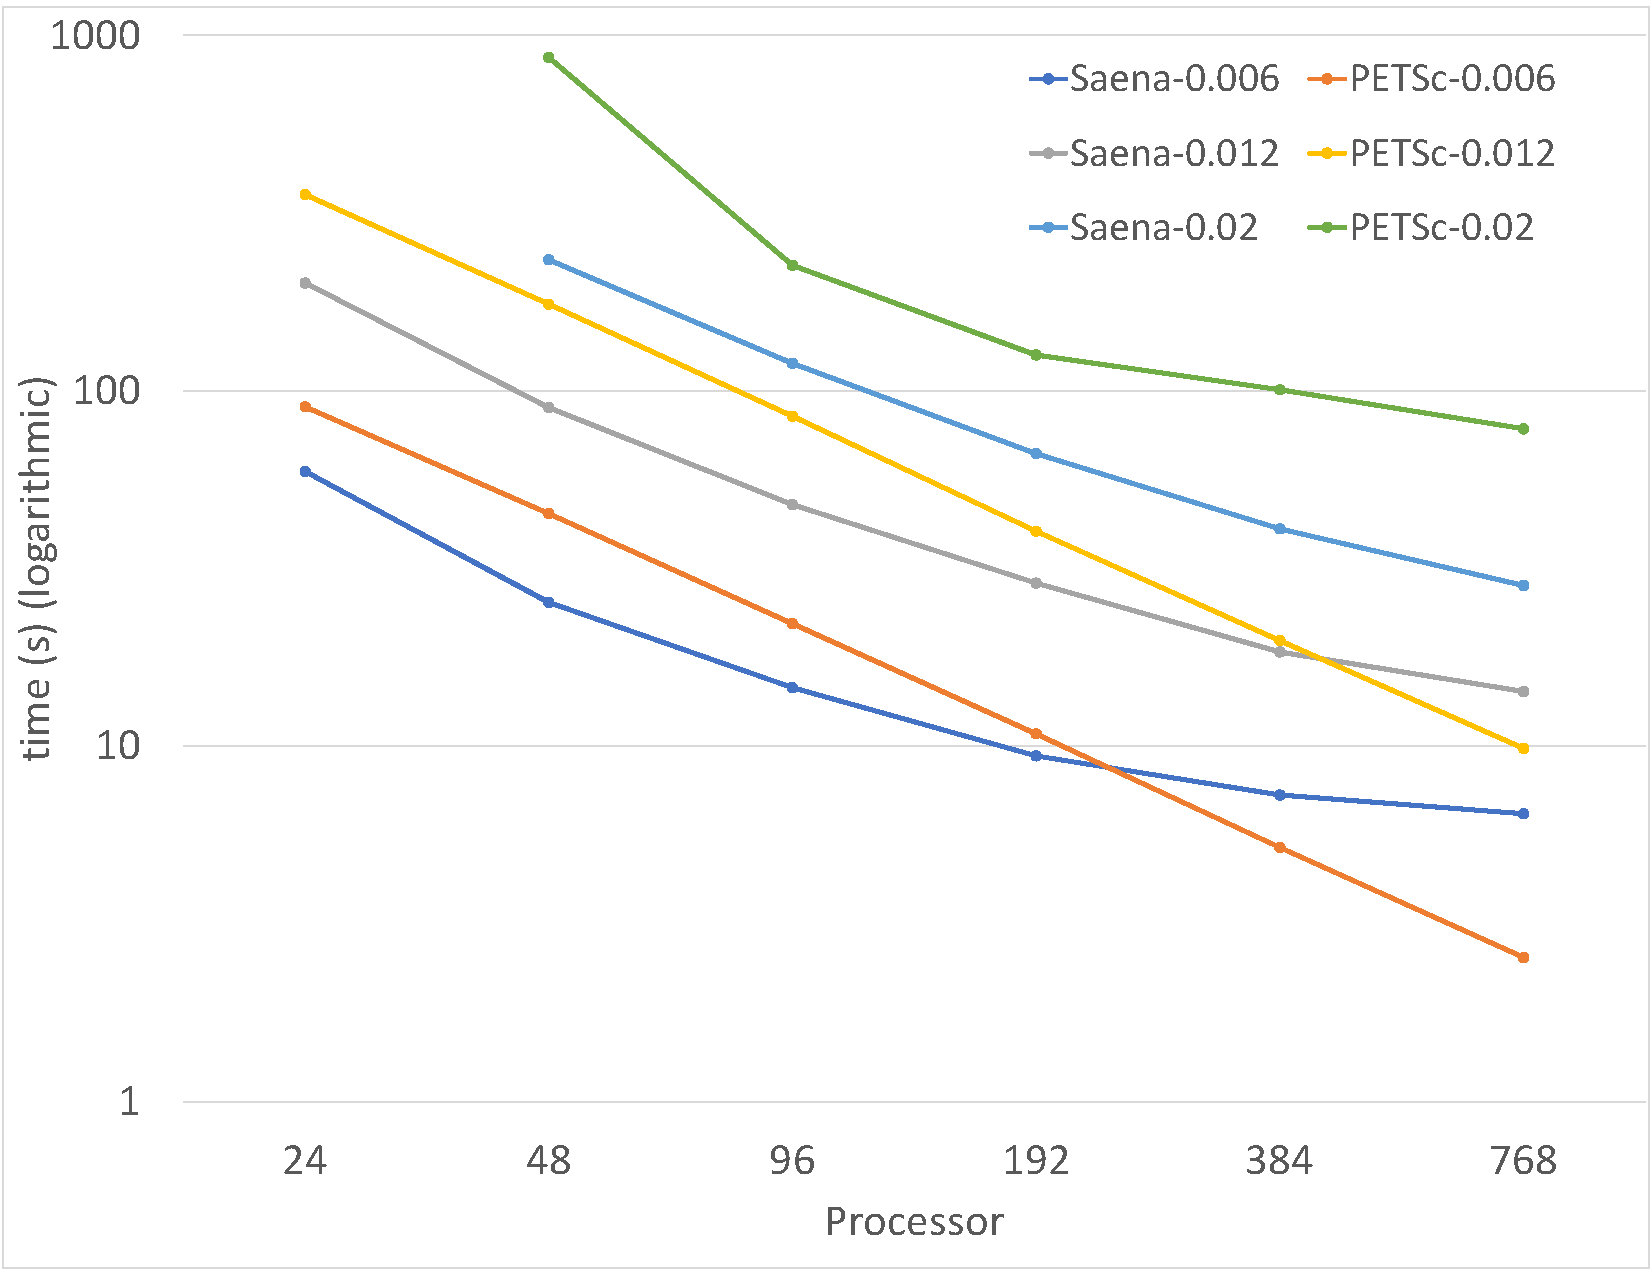
\includegraphics[width=8.5cm,height=4.4cm]{./figures/strong_size_vs_petsc.pdf}
 \caption{Comparison of the the strong scaling between our solver and PETSc. The number for each line shows the density for that matrix. The legend shows the density of each matrix.}
 \label{fig:petsc1}
\end{figure}

Figure\ref{fig:weak1} shows the weak scaling for two banded matrices: one with $24k$ on each node and the other one with $100k$ on each node. Our solver scales better when there is a smaller block of the matrix on each core, which happens when we use more processors or when the matrix is smaller.

\begin{figure}[tbh]
 \centering
 \Description{Description}
 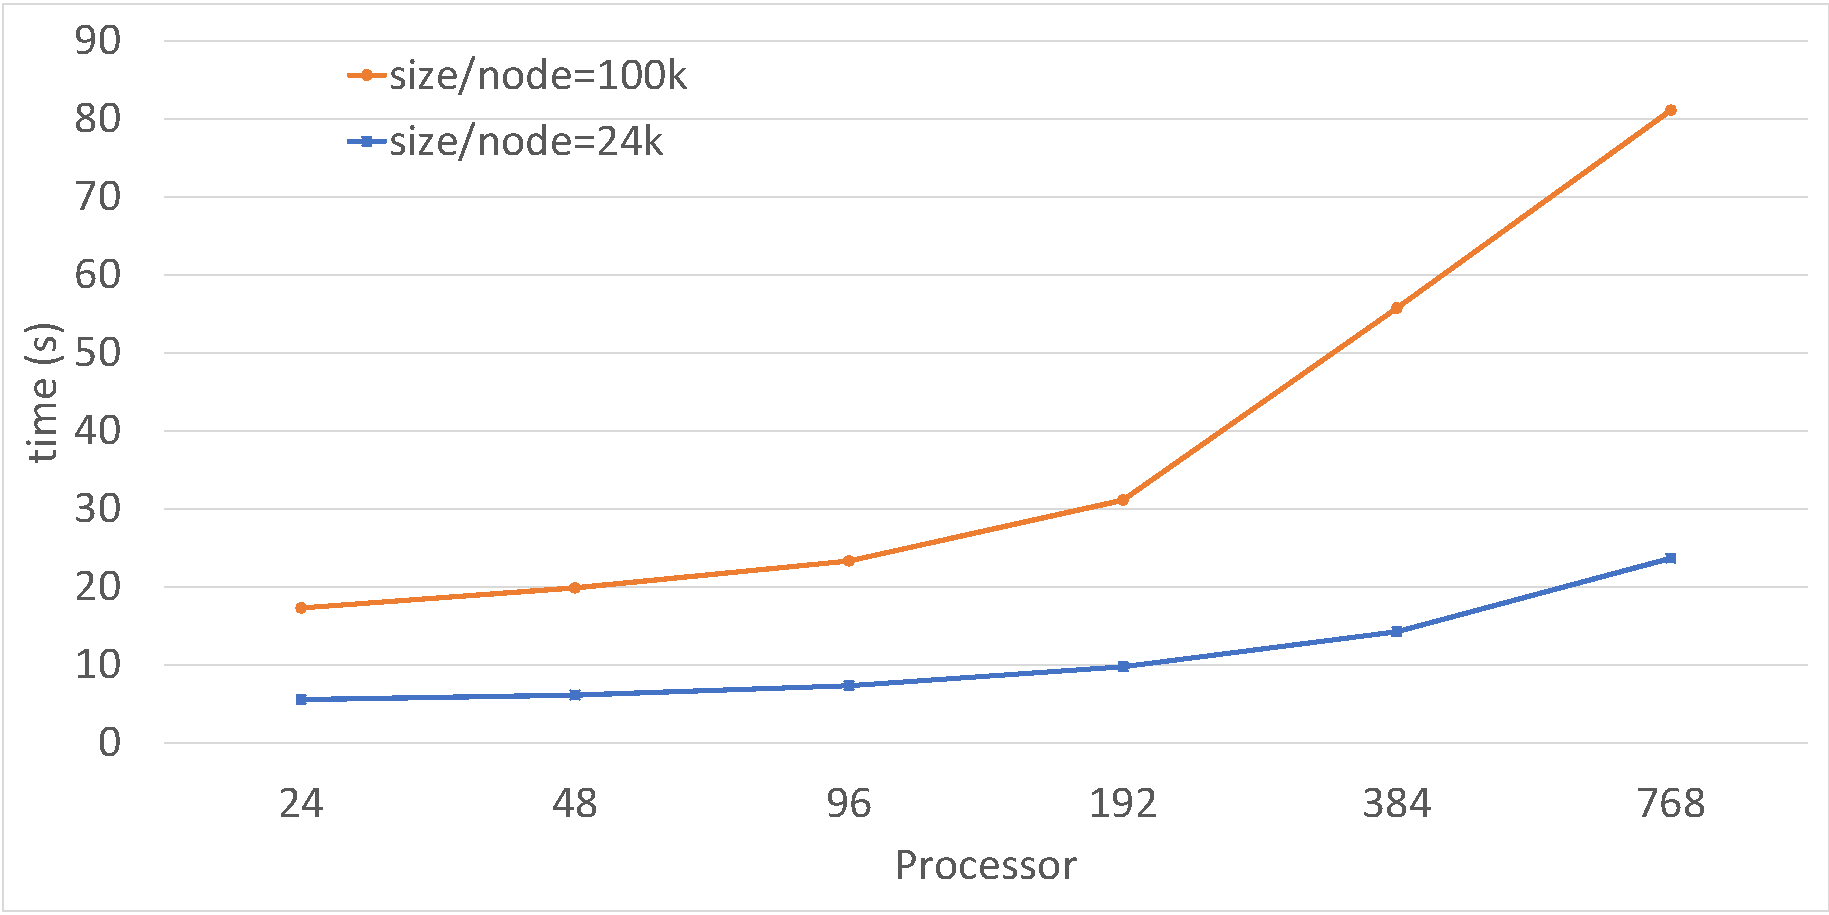
\includegraphics[width=8.5cm,height=4.8cm]{./figures/weak1.pdf}
 \caption{Weak scaling for two banded matrices: blue line shows the one with $24k$ on each node ($1k$ on each core) and red line shows the larger one with $100k$ on each node ($4166$ on each core)}
 \label{fig:weak1}
\end{figure}

\section{Conclusion}
\label{sec:conc}

We have presented a divide and conquer approach to improve the efficiency of matrix-matrix multiplication. We have also designed a low-communication algorithm specific to AMG, to improve the efficiency of the AMG setup phase. We demonstrated performance gains from using our methods and compared our multiplication with the in-built functions within PETSc. In our future work, we want to further improve our performance and scalability and also focus on using sparsification algorithms to ensure the sparsity of coarser levels. 
